% Copyright (c) 2008-2009 solvethis
% Copyright (c) 2010-2011 Casper Ti. Vector
% Public domain.

\chapter{性能测试与评估}\label{chap:envaluation}
本章将对支持物理层WiFi安全研究的验证平台GRTSEC进行评估。
首先在\ref{sec:envaluation_env_setup}节介绍测试环境,介绍开发板型号、开发套件版本号等,
其次在\ref{sec:envaluation_performance}节对GRTSEC的性能进行测试,
然后在\ref{sec:envaluation_demo}节提出多个WiFi安全使用样例,并对GRTSEC在使用样例中的表现进行评测,
最后在\ref{sec:envaluation_summary}节论证了GRTSEC可以满足WiFi安全研究的需求,并且对本章进行总结。

  \section{测试环境}\label{sec:envaluation_env_setup}
  在第四章我们介绍了GRTSEC的前期工作GRT2.0的组成部分,GRTSEC与GRT2.0的组成部分相同,但具体测试环境略有不同。
  在GRTSEC中,我们使用的上位主机是一台支持USB3.0接口、运行有Ubuntu14.04操作系统的计算机,
  FPGA是一块Xilinx VC707板卡\cite{xilinxvc707},
  配置计算机是任意一台支持Xilinx Vivado开发套件的计算机,Windows系统或Linux系统均可,
  射频前端是Analog Device公司的EVAL-AD-FMCOMMS3-EBZ开发板\cite{fmcomms3}。
  FPGA开发工具我们使用的是Xilinx Vivado 2015.2,FPGA嵌入式软件开发工具是Xilinx SDK 2015.2。

  \section{平台性能测试}\label{sec:envaluation_performance}
  本节对GRTSEC平台的性能进行测试,分成两个小节,
  \ref{subsec:envaluation_comparation}小节对GRTSEC与GRT2.0在资源使用率和性能上进行比较,
  \ref{subsec:envaluation_phy_info}小节对GRTSEC在获取物理层信息上的有效性进行测试。

    \subsection{GRTSEC与GRT的对比测试}\label{subsec:envaluation_comparation}
    在本小节我们对GRTSEC与GRT2.0在资源使用率和性能上进行比较。
    GRTSEC相对于GRT2.0在代码上的改动主要有以下几方面:
    	\begin{itemize}
        \item 在物理层中添加AXI接口,打包为IP核,与处理器相连;
    		\item 修改物理层中的同步、频偏、信道估计模块,修改顶层模块,添加物理层信息的三级缓存逻辑及其时钟域转换逻辑;
        \item 修改射频通信库模块,增加回环模式;
    		\item 添加硬件分析模块IP,通过AXI总线与处理器相连;
        \item 修改嵌入式软件代码,增加物理层信息的接口;
        \item 对于使用样例,添加对物理层信息进行数据分析的Python代码。
    	\end{itemize}

    与GRT2.0相比,GRTSEC的代码变化如表\ref{tab:envaluate_code_comparation}所示。
    GRT2.0实现了完整的802.11协议,可以看到,基于GRT2.0进行开发可以付出相对较小的工作量达到目标,体现了GRT2.0的可扩展性。
      \begin{table}[!hbp]
      \centering
      \caption{GRTSEC与GRT2.0的代码比较}
      \label{tab:envaluate_code_comparation}
        \begin{tabular}{|l|p{0.2\textwidth}|p{0.2\textwidth}|l|} \hline
        代码 & GRT2.0的代码行数 & GRTSEC修改或增加代码行数 & 变化比例(\%)\\ \hline
        物理层硬件Verilog代码 & 34233 & 987 & 2.9 \\ \hline
        射频通信库硬件Verilog代码 & 175 & 20 & 11.4 \\ \hline
        硬件分析模块硬件Verilog代码 & / & 130 & / \\ \hline
        嵌入式软件C代码 & 2573 & 44 & 1.7 \\ \hline
        使用样例Python代码 & / & 274 & / \\ \hline
        \end{tabular}
      \end{table}

    下面展示的是FPGA的资源占用率,GRT2.0的资源占有率见表\ref{tab:envaluate_grt2.0_resource},
    增加GRTSEC的扩展后,资源占用率见表\ref{tab:envaluate_grtsec_resource}。
      \begin{table}[!hbp]
      \centering
      \caption{GRT2.0在VC707开发板上的资源占用率}
      \label{tab:envaluate_grt2.0_resource}
        \begin{tabular}{|l|l|l|l|} \hline
        资源 & 已使用 & 总数 & 占用率 \\ \hline
        Flip-Flop & 76781 & 607200 & 12.65 \\ \hline
        LUT & 98657 & 303600 & 32.50 \\ \hline
        Memory LUT & 4551 & 130800 & 3.48 \\ \hline
        I/O & 224 & 700 & 32.00 \\ \hline
        BRAM & 319 & 1030 & 30.97 \\ \hline
        DSP48 & 294 & 2800 & 10.50 \\ \hline
        BUFG & 17 & 32 & 53.12 \\ \hline
        \end{tabular}
      \end{table}

      \begin{table}[!hbp]
      \centering
      \caption{GRTSEC在VC707开发板上的资源占用率}
      \label{tab:envaluate_grtsec_resource}
        \begin{tabular}{|l|l|l|l|} \hline
        资源 & 已使用 & 总数 & 占用率 \% \\ \hline
        Flip-Flop & 79564 & 607200 & 13.10 \\ \hline
        LUT & 95761 & 303600 & 31.54 \\ \hline
        Memory LUT & 4058 & 130800 & 3.10 \\ \hline
        I/O & 224 & 700 & 32.00 \\ \hline
        BRAM & 263 & 1030 & 25.53 \\ \hline
        DSP48 & 303 & 2800 & 10.82 \\ \hline
        BUFG & 14 & 32 & 43.75 \\ \hline
        \end{tabular}
      \end{table}

    Flip-Flop(触发器)和LUT(look-up table,查找表)是Xilinx 7系列FPGA的主要逻辑资源,
    Flip-Flop可用来做寄存器,LUT可用来做逻辑和存储,专门做存储的那部分称作Memory LUT。
    BRAM(Block RAM)是Xilinx 7系列FPGA的主要存储资源,多数FIFO是利用BRAM实现的,
    少数利用DRAM(Distribute RAM)实现,DRAM实际上消耗Memory LUT资源。

    我们可以看到,GRTSEC相对于GRT2.0,Flip-Flop资源使用有所增加但没有增加太多,其他资源如LUT和BRAM资源使用实际上还减少了,
    原因有以下几点:
    	\begin{itemize}
    		\item GRTSEC采用多级寄存器缓存技术进行帧对齐,因此会消耗更多的Flip-Flop,
        但相对于原GRT2.0的消耗只是很小的一部分,所以Flip-Flop使用率增加不多;
    		\item LUT有少量下降,因为原有GRT2.0系统设计中射频部分和LOW MAC都在block design中,
        而中间的物理层在block design之外,GRTSEC将物理层由block design外部移到了block design内部,并封装为一个IP核,
        有效地减少了block design内外部的连线所消耗的LUT资源;
    		\item GRTSEC对系统使用的FIFO进行了优化,减小一些FIFO不必要的深度,因此BRAM和Memory LUT使用率有所下降;
        \item BUFG是用来做时钟分频和去毛刺的,BUFG资源有所下降是因为GRTSEC对全局的时钟进行了优化,
        多处生成同一频率时钟的BUFG合并到一处生成,即相同频率的两个异步时钟合并为一个。
    	\end{itemize}

    然后对嵌入式软件代码的性能进行测试,主要体现在传输延迟上。从收到一帧到回复ACK的时间间隔,是最关键的延迟指标,
    如果延迟太高,会大大影响传输性能,留给用户可编程的空间会降低。
    GRTSEC相对GRT2.0增加了读取物理层信息的过程,本节对GRTSEC在这方面增加的负载进行了测量,
    测量方法是记录不读取物理层信息时软件代码执行时间,即GRT2.0的软件代码执行时间,再记录读取物理层信息时的软件代码执行时间,
    即GRTSEC的软件代码执行时间,多帧测量求平均后再做差。
    此处的软件代码代码执行时间是嵌入式软件处理一帧的总时间,包括了等待硬件计算CRC校验的时间,接收帧越长此时间越长,
    差值即为读取物理层信息所花的时间。
    性能结果见表\ref{tab:envaluate_grtsec_latency}。
    \begin{table}[!hbp]
    \centering
    \caption{GRTSEC与GRT2.0的延迟性能对比表}
    \label{tab:envaluate_grtsec_latency}
      \begin{tabular}{|l|l|l|} \hline
      测量对象 & 接收帧数 & 平均软件处理时间(us) \\ \hline
      GRT2.0软件接收端 & 3219 & 41.801802 \\ \hline
      GRTSEC软件接收端 & 3641 & 41.867069 \\ \hline
      读取物理层信息 & / & 0.065268 \\ \hline
      \end{tabular}
    \end{table}

    我们可以看到,延迟增加约65ns,增加的并不多,因为经过精心设计的硬件逻辑,可以保证在软件读取之前将物理层信息准备好,
    因此多花的时间即为读取多组AXI寄存器的时间,硬件开销很小。

    \subsection{GRTSEC获取物理层信息性能测试}\label{subsec:envaluation_phy_info}
    本小节对GRTSEC读取物理层信息的有效性进行测试,选用真实的802.11设备进行测试,地点是北京大学理科五号楼五楼。
    我们在2.4GHz频段的最常用1信道(2.412GHz)以及5GHz频段的161信道(5.805GHz),对该频段进行1-2分钟的监听,
    记录频偏、CSI、RSSI、调制方式等物理层信息,绘制成以下图表。
    这些图表的目的是展示GRTSEC读取物理层信息的有效性,WiFi安全的研究者可以物理层信息进行进一步地分析和处理,本文不做更多的分析。

      \begin{table}[!hbp]
      \centering
      \caption{1信道设备分布及频偏值表}
      \label{tab:envaluate_2412_frame_number}
        \begin{tabular}{|l|l|l|l|l|} \hline
        序号 & 设备MAC地址前12位 & 接收帧数 & 频偏平均值(rad) & 频偏标准差(rad) \\ \hline
        设备1  & 0x003A98 & 4247 & -26.5586 & 6.8343 \\ \hline
        设备2  & 0xA0C589 & 686  & 5.0964 & 6.7770 \\ \hline
        设备3  & 0xA434D9 & 556  & -24.5785 & 7.6319 \\ \hline
        设备4  & 0x66C002 & 507  & -0.1805 & 4.3990 \\ \hline
        设备5  & 0x48437C & 409  & -11.0173 & 5.1095 \\ \hline
        设备6  & 0x08D40C & 394  & 0.3264 & 3.7925 \\ \hline
        设备7  & 0x2ADCB6 & 364  & -1.1527 & 11.1968 \\ \hline
        设备8  & 0xDE436A & 229  & -27.3364 & 3.3673 \\ \hline
        设备9  & 0x8AF314 & 195  & -24.1565 & 6.2982 \\ \hline
        设备10 & 0xF48B32 & 151  & 6.2376 & 7.9951 \\ \hline
        其它设备 & /      & 1218 & -15.9206 & 13.1757 \\ \hline
        \end{tabular}
      \end{table}

    表\ref{tab:envaluate_2412_frame_number}为1信道下接收帧的设备分布及其频偏值,
    可以看到,不同设备之间频偏相差较大,除设备7外,同一设备的频偏标准差小,其它一行的频偏标准差大,进一步说明不同设备之间频偏相差较大。

      \begin{table}[!hbp]
      \centering
      \caption{161信道设备分布及频偏值表}
      \label{tab:envaluate_5805_frame_number}
        \begin{tabular}{|l|l|l|l|l|} \hline
        序号 & 设备MAC地址前12位 & 接收帧数 & 频偏平均值(rad) & 频偏标准差(rad) \\ \hline
        设备A  & 0xDCEF09 & 4953 & -4.8232 & 9.7126 \\ \hline
        设备B  & 0x9DA868 &  711 & -3.4210 & 4.7535 \\ \hline
        设备C  & 0x67A622 &  672 & -4.0277 & 7.7692 \\ \hline
        设备D  & 0x9AE07C &  291 & -3.7384 & 8.9364 \\ \hline
        设备E  & 0xD6FF00 &  189 & -3.9803 & 5.4527 \\ \hline
        设备F  & 0xB699D3 &   83 & -2.8351 & 1.9508 \\ \hline
        设备G  & 0x7ADC74 &   83 & -62.3400 & 24.0868 \\ \hline
        设备H  & 0x2C9FC7 &   56 & -5.5038 & 13.2189 \\ \hline
        其它设备 & /      &  575 & -18.3011 & 37.5738 \\ \hline
        \end{tabular}
      \end{table}

    表\ref{tab:envaluate_5805_frame_number}为161信道下接收帧的设备分布及其频偏值,
    在5GHz频段下,设备7与其它设备之间频偏相差很大,
    相比2.4GHz,其它一行的频偏标准差非常大,达到了37,进一步说明不同设备之间频偏相差较大。

    图\ref{fig:envaluation_csi_2_4g}与图\ref{fig:envaluation_csi_5g}分别展示了在2.4GHz和5GHz下两台设备的CSI随时间的变化,
    两台设备分别是前面提到的两个信道下出现最多的设备,接收帧数分别为4247帧和4953帧,监听时间都在10秒以上,
    选取了CSI中两个子载波-21与+21的幅度响应进行展示,这两个子载波也是802.11协议中规定的导频子载波。
    由两个图可以看到,除去因环境变化引起骤降和骤增,总体幅度响应的趋势是缓慢变化的。
  		\begin{figure}[H]
  			\centering
  			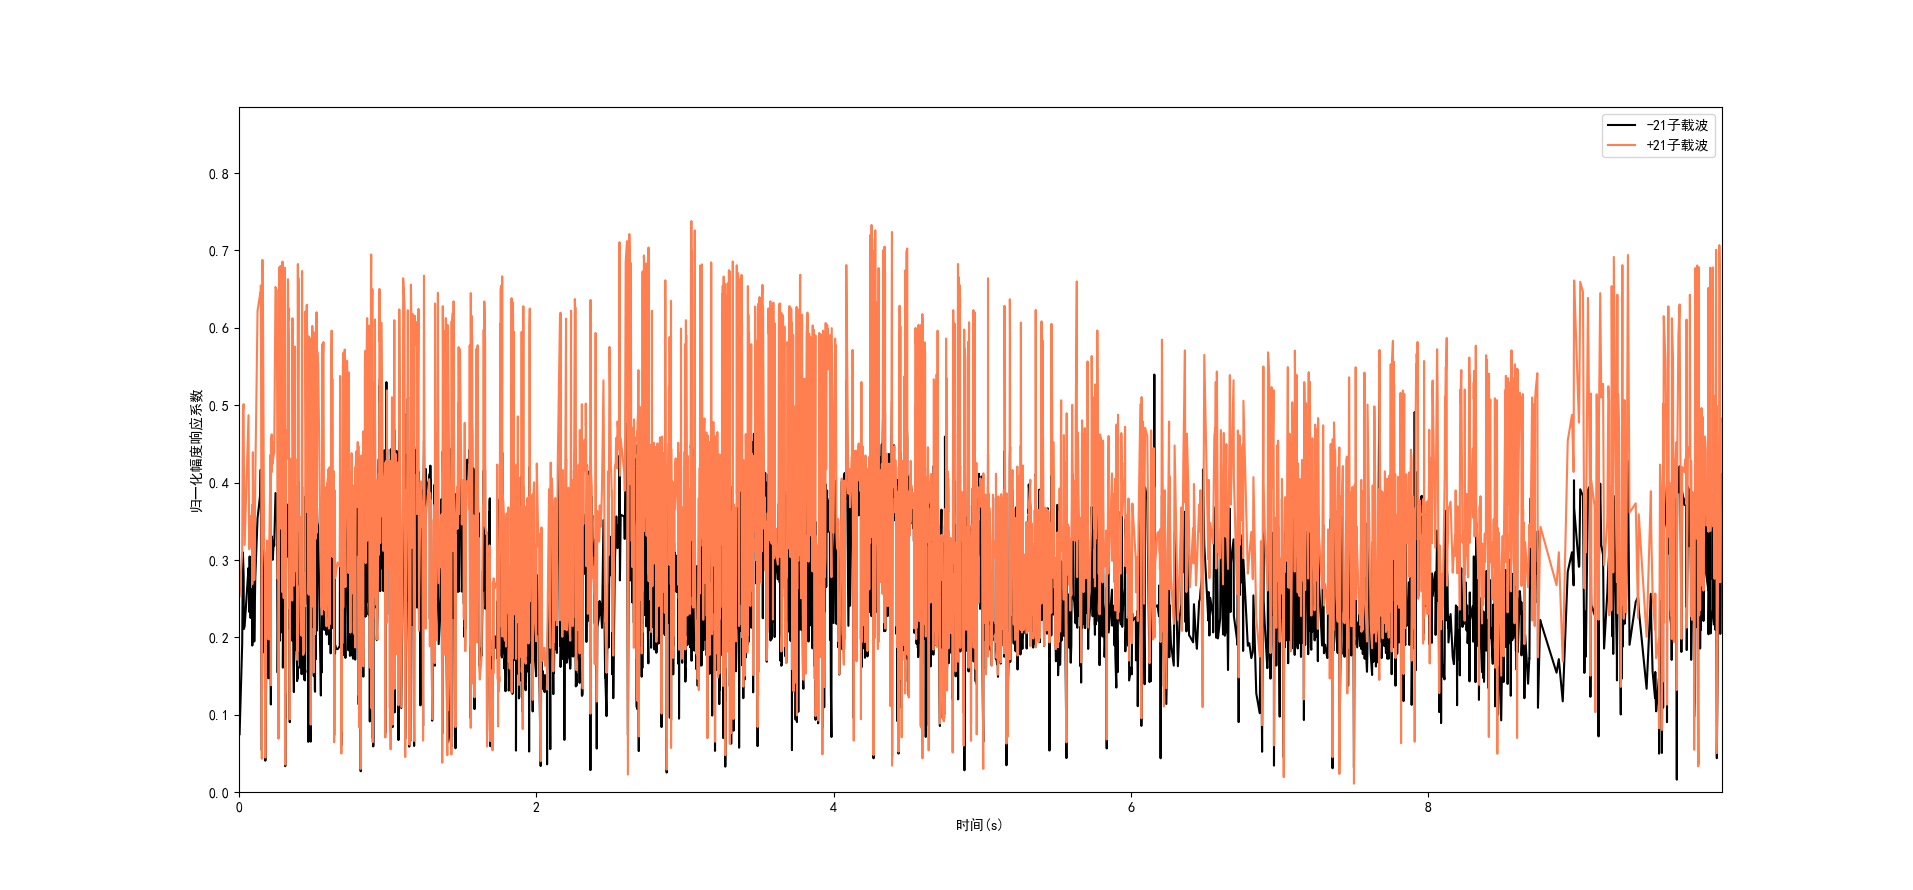
\includegraphics[width=1.0\textwidth]{img/envaluation_csi_2_4g.png}
  			\caption{2.4GHz下某设备子载波幅度响应曲线}
  			\label{fig:envaluation_csi_2_4g}
  		\end{figure}

  		\begin{figure}[H]
  			\centering
  			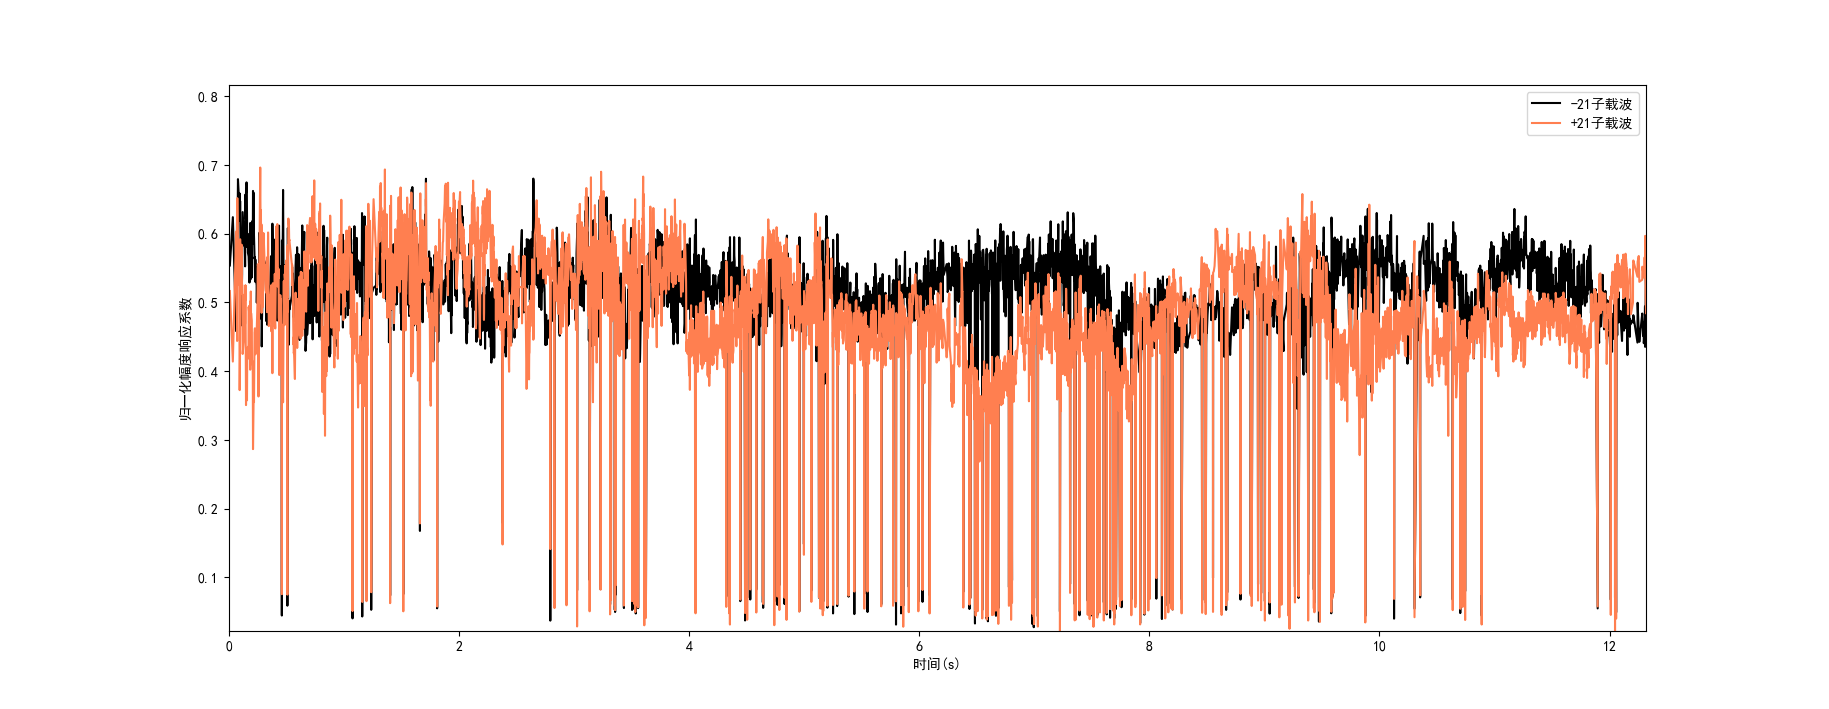
\includegraphics[width=1.0\textwidth]{img/envaluation_csi_5g.png}
  			\caption{5GHz下某设备子载波幅度响应曲线}
  			\label{fig:envaluation_csi_5g}
  		\end{figure}


    图\ref{fig:envaluation_rssi_2_4g}与图\ref{fig:envaluation_rssi_5g}分别展示了在2.4GHz和5GHz下各两台设备的RSSI随时间的变化,
    记录的是前面提到的两个信道下出现最多的两台设备,2.4GHz下是设备1和设备2,5GHz下是设备A和设备B。
    可以看到2.4GHz下的两台设备的RSSI差别较大,5GHz下的这两台设备RSSI差别较小。
  		\begin{figure}[H]
  			\centering
  			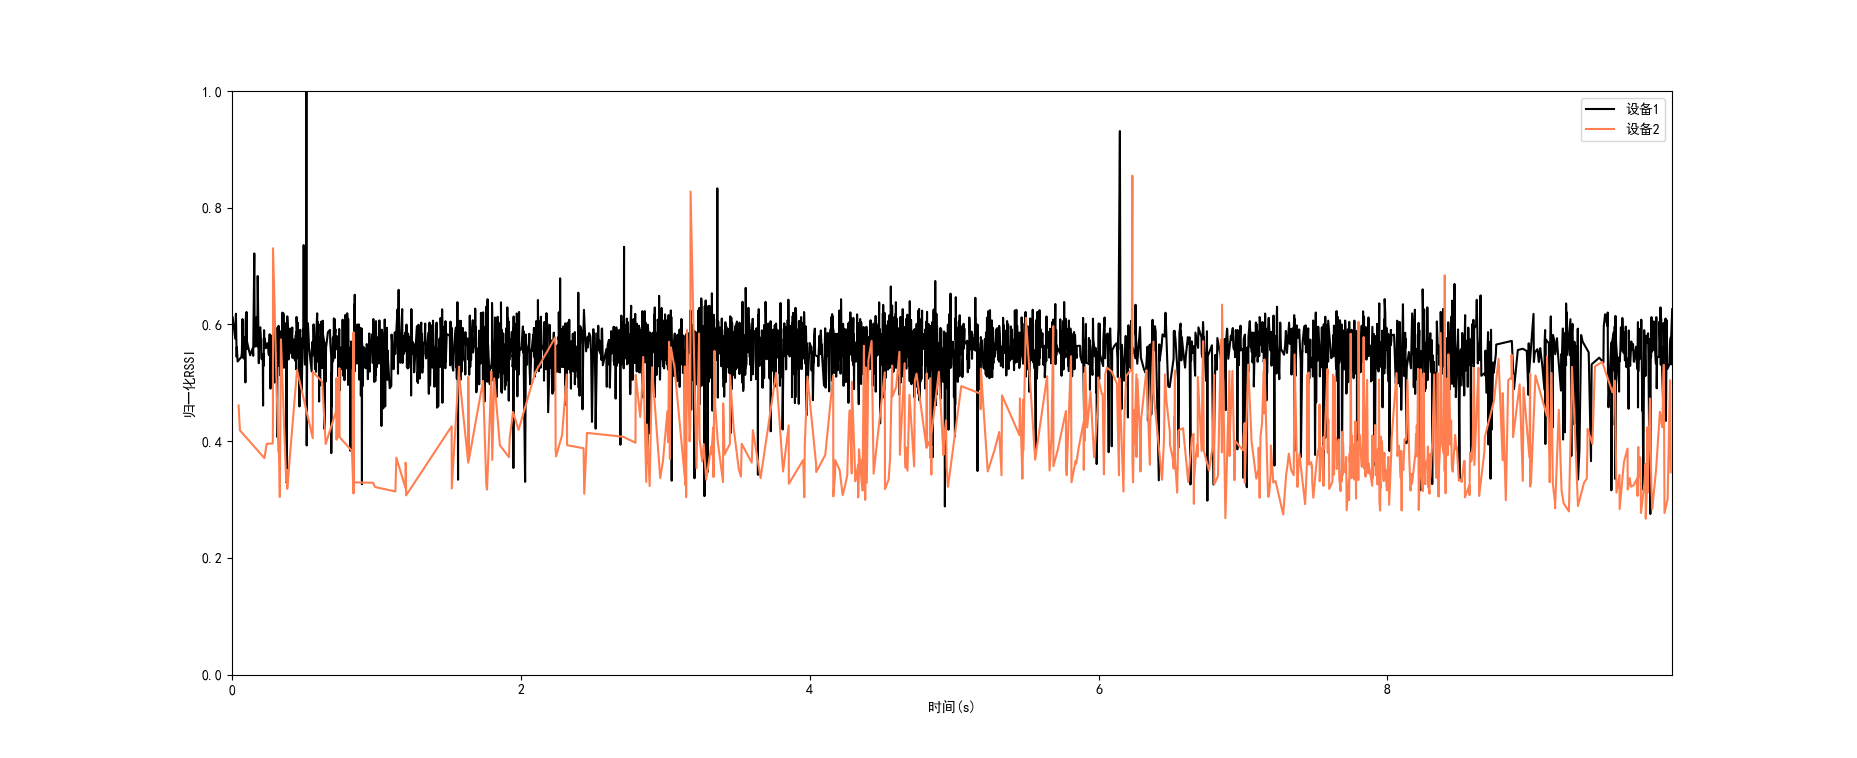
\includegraphics[width=1.0\textwidth]{img/envaluation_rssi_2_4g.png}
  			\caption{2.4GHz下两台设备RSSI随时间变化曲线}
  			\label{fig:envaluation_rssi_2_4g}
  		\end{figure}

  		\begin{figure}[H]
  			\centering
  			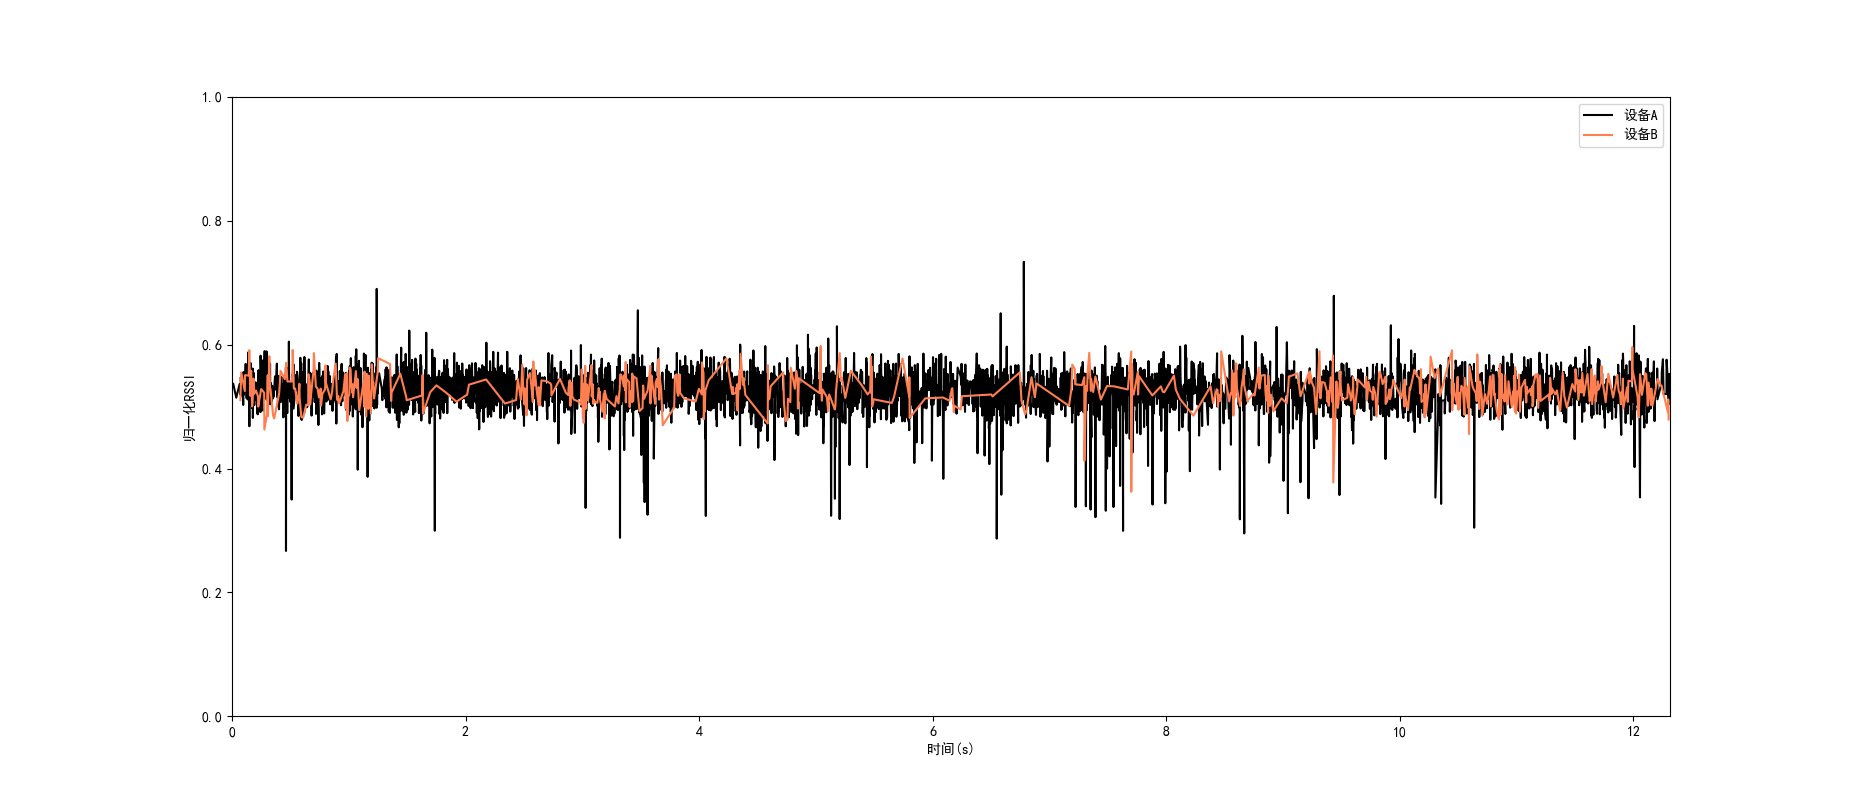
\includegraphics[width=1.0\textwidth]{img/envaluation_rssi_5g.png}
  			\caption{5GHz下两台设备RSSI随时间变化曲线}
  			\label{fig:envaluation_rssi_5g}
  		\end{figure}

    以上呈现的只是一部分测试数据的简单分析结果,目的是展示GRTSEC对物理层信息的提取能力,
    实际上在第\ref{chap:background}章提到,物理层信息在WiFi安全的研究中有广泛的应用,待GRTSEC平台的使用者去发掘。

  \section{样例测试}\label{sec:envaluation_demo}
	本节会通过两个实际的物理层WiFi安全研究的样例,进一步说明GRTSEC平台的使用场景和方法,
	同时,用户也可以基于这些使用样例开展自己的研究。
	在\ref{subsec:demo_fake_wifi}小节会介绍如何使用GRTSEC搭建伪装WiFi,并用伪装WiFi发起钓鱼攻击,获取用户的敏感信息,
	在\ref{subsec:demo_phy_auth}小节会提出一种利用利用硬件指纹技术对不同WiFi设备进行识别的方法。

    \subsection{搭建伪装AP}\label{subsec:demo_fake_wifi}

    身份伪装是很多WiFi攻击的前提和基础,比如DoS攻击、会话劫持、中间人攻击、数据篡改、窃听等\cite{ieeewc10noncryp}。
    针对身份伪装的安全研究需要先搭建伪装AP,本节设计了搭建伪装AP的样例,并用伪装AP发起钓鱼攻击,获取用户的敏感信息。
    下面将通过一个实际的例子说明伪装AP的用途。

		在北京大学,计算中心为全校师生员工提供了无线校园WiFi,名字是Wireless PKU,遍布教学楼、实验室、食堂等场所。
		Wireless PKU是无密码的开放WiFi,用户连接到Wireless PKU后,首先跳转到一个认证网页,输入网关的账号、密码进行登录,
		登录后才可以继续上网。对于学生来说,网关账号、密码同时也是其他校园网页登录的账号、密码,
		包括信息登记、成绩查询、选课申请等都使用同一套认证系统。
		假如密码泄露会造成巨大的损失,轻则已选的课程被退掉或者成绩泄露,重则学籍信息被篡改,无法毕业。
		在本小节,我们将利用GRTSEC搭建AP,伪装成Wireless PKU,并制作一个钓鱼认证网页,用来盗取统一认证账号。

		真实Wireless PKU的AP与伪装AP的分布场景如图\ref{fig:demo_fake_wifi_scenary}所示,
		这张图真实地模拟了北京大学理科五号楼五楼的AP分布,其中AP1、AP2、AP3是北京大学计算中心布置的Wireless PKU的AP,
		GRTSEC摆放在房间1中。假设AP1、AP2、AP3的MAC地址是$MA_1$、$MA_2$、$MA_3$。
		房间1内有个用户,我们称他为小明,在GRTSEC发起伪装之前,小明可以看到信号较强的AP1和信号弱一些的AP2,看不到远处的AP3。
		为了让小明能够连接上GRTSEC,我们将GRTSEC的SSID设置为Wireless PKU,将MAC地址设置为$MA_3$,
		即使小明用MAC地址的白名单来分辨伪装AP也是无法识别的。小明连接上GRTSEC搭建的AP后,会先看到钓鱼认证网页,
		习惯了上网认证的小明会毫无戒心的输入自己的统一认证账号和密码。

		此样例旨在说明设计目标中的两点:可与商用802.11设备实时通信,在这里是与小明的手机相连;
		可与上层网络协议栈连接,在这里是与应用层的钓鱼认证网页相连。

			\begin{figure}
				\centering
				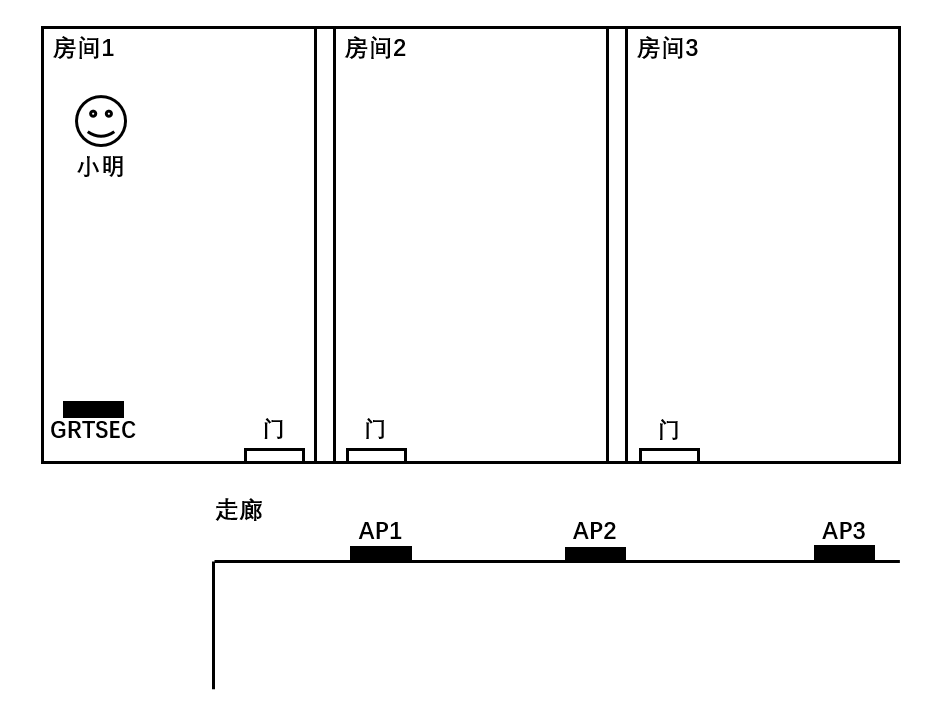
\includegraphics[width=0.7\textwidth]{img/demo_fake_wifi_scenary.png}
				\caption{伪装AP与真实AP分布场景图}
				\label{fig:demo_fake_wifi_scenary}
			\end{figure}

		具体实现时,首先,在上位主机上搭建钓鱼认证网页,钓鱼网页参考了本组张高瀚同学做的网页\cite{zgh17wifi},
		然后,修改主机的网络配置,使网络请求都转跳到钓鱼认证网页,
		最后,将GRTSEC运行在AP模式,等待进入房间1的用户连接。

    下面将通过实际测试结果说明其有效性。
    如图\ref{fig:envaluation_fake_ap}所示,我们利用GRTSEC搭建伪装AP,名字为Wireless PKU GRTSEC,
    可以被一部手机连接,手机自动可以跳转到钓鱼页面。
  		\begin{figure}[H]
  			\centering
  			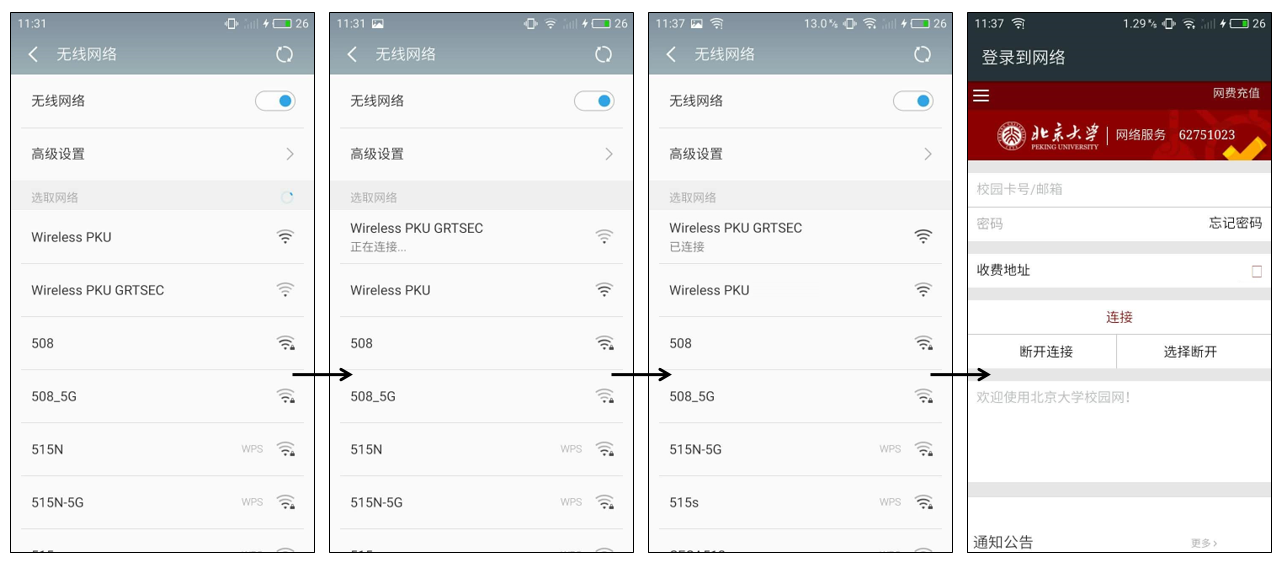
\includegraphics[width=1.0\textwidth]{img/grtsec_fake_ap.png}
  			\caption{伪装AP与钓鱼认证网页}
  			\label{fig:envaluation_fake_ap}
  		\end{figure}

    使用WiFi信号分析工具WirelessMon\cite{wirelessmon}对周边WiFi进行查看,如图\ref{fig:envaluation_fake_ap_wirelessmon},
    可以看到Wireless PKU和Wireless PKU SEC同时存在,且Wireless PKU SEC的MAC地址伪装成了与AP3的MAC地址,与AP1、AP2的MAC地址很相近。
  		\begin{figure}[H]
  			\centering
  			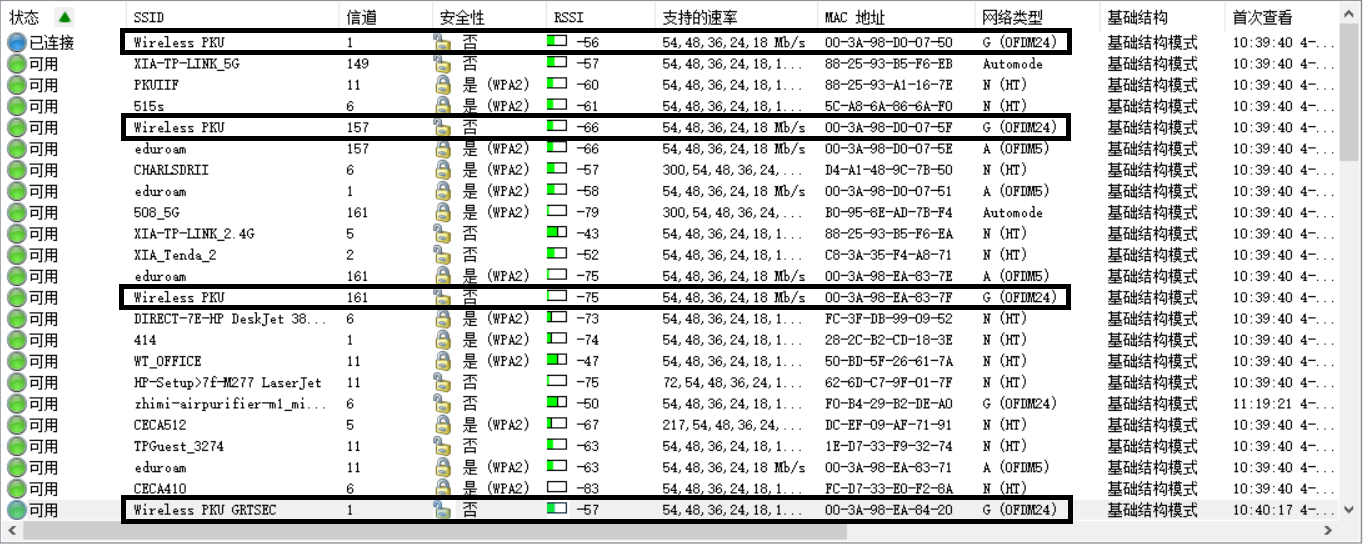
\includegraphics[width=1.0\textwidth]{img/grtsec_wirelessmon.png}
  			\caption{使用WirelessMon查看伪装AP}
  			\label{fig:envaluation_fake_ap_wirelessmon}
  		\end{figure}

    我们可以看到,使用GRTSEC搭建的伪装AP足够以假乱真。
    用户手机真实连上了GRTSEC搭建的伪装AP,说明GRTSEC可与商用设备实时通信,
    用户手机看到了钓鱼认证网页,说明GRTSEC兼容上层网络应用。

    \subsection{利用物理层信息识别不同WiFi设备}\label{subsec:demo_phy_auth}
  	在802.11协议中,WiFi身份的标识是MAC地址,然而MAC地址非常容易伪装,利用笔记本电脑,
  	或者一部root过的安卓手机,搭配一些软件工具,就可以任意修改自己的MAC地址\cite{NetworkSecurity11hacking}。
  	% 在本节,我们提出一种利用物理层信息识别WiFi设备的方法,具体来说,使用物理层信息中的频偏和时钟偏移,识别不同的WiFi设备硬件,
  	% 弥补仅靠MAC地址进行识别的缺陷。

		下面通过一个实际的例子说明利用物理层信息识别不同WiFi设备的用途。
    一些用户家里的WiFi偶然被邻居知道了密码,又不想修改密码使自己的全部设备重新输入一次,我们假设这样的一个用户叫小明。
		为了防止邻居的“蹭网”,小明会对路由器进行设置,只允许特定MAC地址的设备连接,目前很多路由器支持这种模式。
		但是,不怀好意的邻居可以监听到小明设备的MAC地址,将自己的设备伪装成小明的设备骗过路由器,继续进行蹭网。
		小明希望做的是对自己的设备进行信任而不是对MAC地址进行信任,在本节,我们利用GRTSEC从接收到的包中提取频偏和时钟偏移,
		生成与WiFi设备对应的硬件指纹,这样小明可以在路由器端选择对特定硬件指纹进行信任,防止邻居继续蹭网。

		本样例主要关注对不同WiFi设备的识别和区分,并不针对无线路由器识别用户设备,实际上这种方法是通用的,
		可用于AP识别STA,可用于识别\ref{subsec:demo_fake_wifi}节提出的伪装AP,也可用于STA之间的互相识别。

      \begin{table}[!hbp]
      \centering
      \caption{不同的STA的频偏值}
      \label{tab:envaluate_freq_offset}
        \begin{tabular}{|l|l|l|l|} \hline
        设备 & 接收帧数 & 频偏平均值(rad) & 频偏标准差(rad) \\ \hline
        华为手机 & 451 & 14.8190 & 2.9401 \\ \hline
        iPhone & 223 & -29.0859 & 2.8856 \\ \hline
        小米手机 & 512 & 9.8436 & 2.3449 \\ \hline
        \end{tabular}
      \end{table}

      \begin{table}[!hbp]
      \centering
      \caption{利用机器学习方法识别不同的STA}
      \label{tab:envaluate_identify_sta}
        \begin{tabular}{|l|l|} \hline
        模型或算法 & 正确率(\%) \\ \hline
        k最近邻算法 & 98.15 \\ \hline
        线性回归分析 & 98.48 \\ \hline
        随机森林算法 & 97.31 \\ \hline
        决策树回归 & 96.80 \\ \hline
        支持向量机 & 97.98 \\ \hline
        \end{tabular}
      \end{table}

		下面介绍具体实现。
    首先,我们利用GRTSEC监听周边WiFi设备发出的包,记录物理层信息频偏和MAC地址;
		然后,我们将该帧的频偏值和MAC地址作为一个组合,前半部分数据用来训练机器学习模型,
    使用的机器学习模型有k最近邻算法(k-NearestNeighbor,KNN)、
    线性回归分析、随机森林算法、决策树回归、支持向量机(Support Vector Machine,SVM);
		最后,我们将记录到的后半部分数据作为测试集,用训练好的模型进行区分。
		训练和测试代码都由Python实现,使用的机器学习库是目前最常用的开源Python机器学习框架scikit-learn\cite{sklearn}。

    下面介绍测试结果。我们对三台设备进行监听,使用的训练集组数为1186组,多组数据求平均,
    频偏结果如\ref{tab:envaluate_freq_offset}所示。三部设备分别为华为荣耀6p、iPhone4s、小米Note。

    可以看到,不同设备之间的频偏差别很大,而且标准差不大,作为用来识别设备的参数非常合适。
    我们使用的测试集组数为594组,测试结果如表\ref{tab:envaluate_identify_sta}所示。
    可以看到,无论使用机器学习哪种模型,正确率都在96\%以上。

    以上实验表明,通过物理层信息频偏对不同设备进行识别,正确率较高,
    这种方法可以在多种场景下进行应用,例如:
			\begin{itemize}
				\item 区别不同的STA,使手机和笔记本电脑工作在STA模式,用GRTSEC对这些设备进行区分,
				应用场景是本节提到的防邻居“蹭网”;
				\item 区别不同的AP,在同一地点存在多个同SSID的AP,用GRTSEC进行区分,
				应用场景是识别\ref{subsec:demo_fake_wifi}节提出的伪装AP;
				\item 识别不同地点的AP,网络服务商在不同地点布置AP,例如校园网,用户设备可以通过AP进行定位。
			\end{itemize}

    上述样例使用频偏对不同设备进行识别,不区分AP和STA,实际上对于不同AP之间的识别,可以用时钟偏移这个物理层信息。
    有研究利用AP发出的beacon包的时间间隔,推算出不同AP设备的时钟偏移\cite{tmc10clock}。
    GRTSEC提供了精确到10ns的帧时间戳,完全可以支持此类研究。
		区别不同的STA时,由于STA不会定时发送beacon包,我们无法获得时钟偏移,只能得到频偏,无法使用此方法。

  \section{讨论与总结}\label{sec:envaluation_summary}
  本章对支持物理层WiFi安全研究的验证平台GRTSEC进行了评估,对测试结果进行了呈现。
  下面我们对GRTSEC满足设计目标进行论证。

  在第\ref{chap:demand}章我们针对三种WiFi安全研究,模拟WiFi攻击、基于加密的安全机制、基于身份验证的安全机制,
  总结了对无线验证平台的需求,提出了设计目标:可与商用802.11网卡实时通信,可自定义物理层和MAC层的数据处理流程,
  方便获取物理层信息,支持安全算法的软硬件实现,兼容上层网络协议。
  在前期工作GRT2.0系统中,通过高性能射频通信库的设计以及团队的工作,达到了与商用802.11网卡实时通信、可自定义物理层和MAC层的数据处理流程、
  兼容上层网络协议的目标。在GRTSEC的设计中,我们提供了一套物理层信息的提取与软硬件编程的框架,
  达到了方便获取物理层信息、支持安全算法的软硬件实现的目标。

  结合测试结果,\ref{sec:envaluation_performance}节的平台测试结果表明,GRTSEC提取物理层信息是高效且有效的,
  在占用资源较少、对软件性能影响低的前提下,提供了多种常见的物理层信息,在实际通信环境中收集这些物理层信息并进行了数据的简单处理。
  \ref{sec:envaluation_demo}节提供了两个使用样例,搭建伪装WiFi的使用样例进一步说明了GRTSEC可以模拟WiFi身份伪装攻击,
  兼容上层网络协议栈,利用物理层信息识别不同WiFi设备的样例对一个实际的WiFi安全研究进行验证,
  验证结果一方面说明这种安全策略是可行的,另一方面也论证了GRTSEC在安全研究中具有实际的使用价值。
  GRTSEC还提供了软硬件数据处理的框架,例如对于基于加密的安全机制,用户可以先通过软件验证加密算法正确性,再通过我们提供的硬件分析模块实现算法,
  对加密解密过程进行加速,在实际通信环境中加以验证。
  总的来说,GRTSEC作为一种支持物理层WiFi安全研究的验证平台,可以满足WiFi安全研究者的需求
